\documentclass[a4paper]{cours-bdd}

\cristal

\title{COVID Simulation}

\begin{document}

\frame{\titlepage}


% --------------------------------------


\begin{frame}
  \hfill \
  \begin{center}
    \Huge
    Préambule
  \end{center}
  \hfill \

\end{frame}



% --------------------------------------

\begin{frame}[fragile]
  \frametitle{Modéliser les épidémies : pour faire quoi ?}

  Aider à comprendre.\\
  Aide à la décision.\\
  Essayer de répondre aux grandes questions. \\
  \begin{itemize}
  \item Combien de temps va durer l’épidémie ?
  \item Combien de personnes seront infectées au cours de la crise ? 
  \item Combien de personnes décèderont au cours de la crise ? 
  \item Combien de personnes doivent être immunisées ?
  \item Quand mettre en place un ou des confinements ?
  \item Quelle durée doivent avoir les confinements ?
  \item Quand arrivera t-on à saturation des hopitaux ?
  \end{itemize}
  
\end{frame}

% --------------------------------------

\begin{frame}[fragile]
  \frametitle{Principe}

  Ne jamais perdre de vue que  :
  \begin{itemize}
  \item Un modèle n'est qu'une abstraction de la réalité
  \item L'important n'est pas d'avoir le plus de paramètres, mais de trouver les plus pertinents (l'essence du problème étudié)
  \item Pour que les thématiciens accaparent un modèle, il faut qu'il soit simple (exemple le modèle SIR : 3 boite cité dans des centaines de travaux en épidémio)
  \end{itemize}

  \bigskip
  
  \begin{block}{}
    \begin{center}
  Torturez un modèle, il finit toujours par avouer !
\end{center}
\end{block}

\end{frame}

  
% --------------------------------------

\begin{frame}[fragile]
  \frametitle{Différentes approches}

  %\fbox{}
  \begin{minipage}[b]{0.45\columnwidth}
    \vspace{0.0cm}
    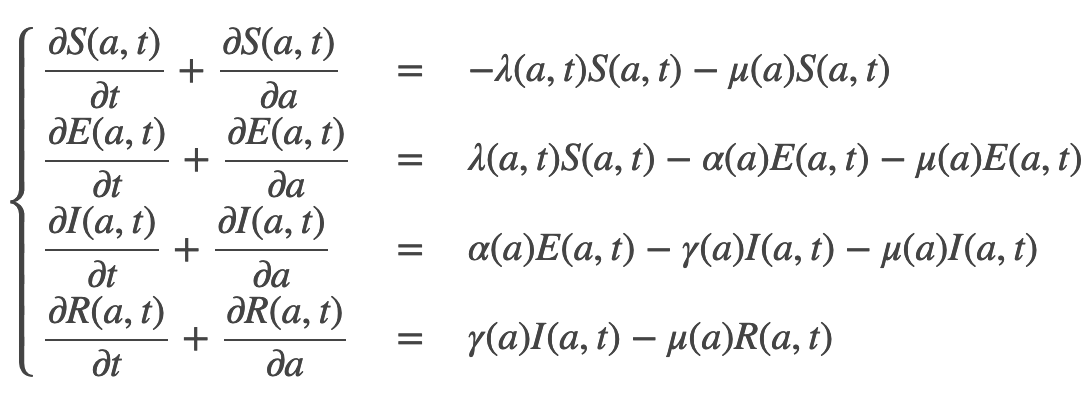
\includegraphics[width=\linewidth]{approcheMath.png} \\
    Approche Mathématique 
      \end{minipage}    
  \hfill \ 
  \begin{minipage}[b]{0.45\columnwidth}
        \vspace{0.0cm}
        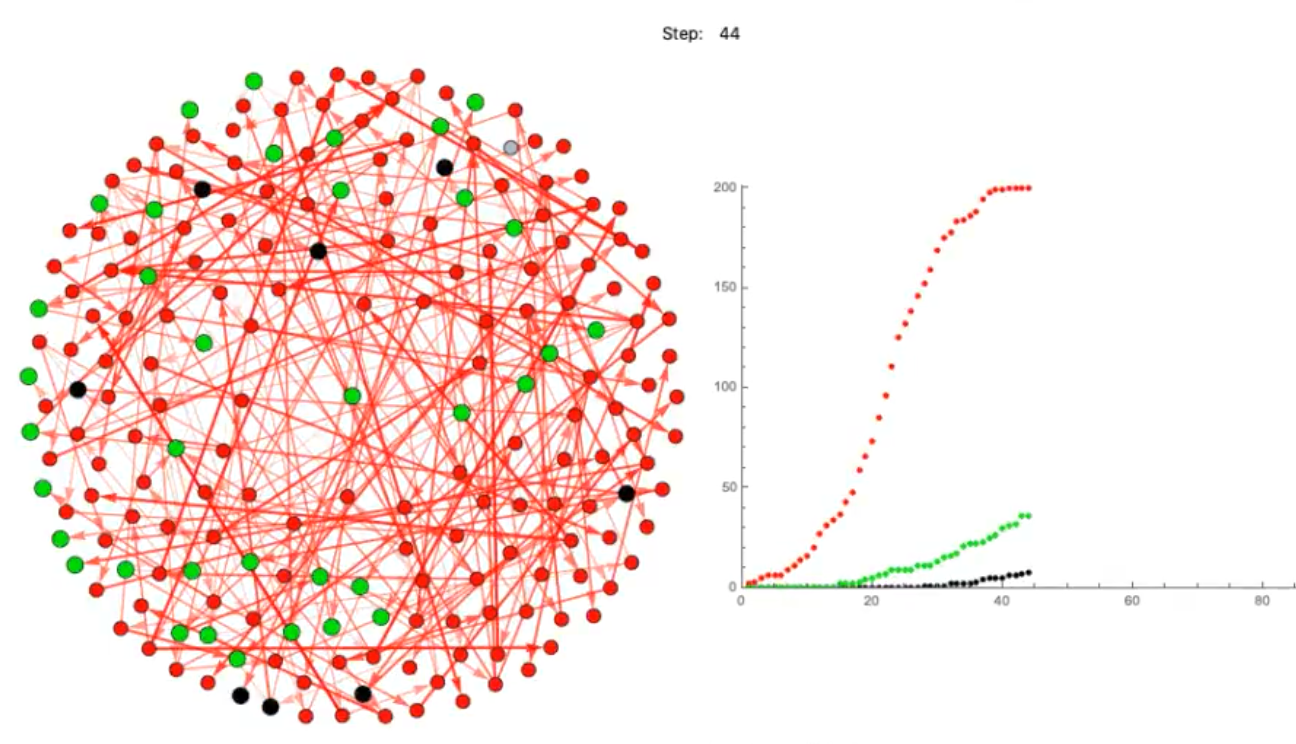
\includegraphics[width=0.8\linewidth]{approcheNetwork.png} \\
        Approche par réseaux sociaux
      \end{minipage}
      \ 

  \begin{minipage}[t]{0.45\columnwidth}
        \vspace{0.0cm}
        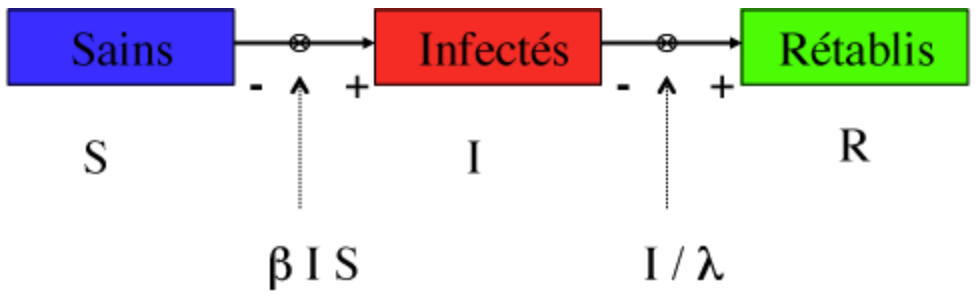
\includegraphics[width=\linewidth]{modeleSIR.png} \\
        Approche par flux
  \end{minipage}
  \hfill \
  \begin{minipage}[t]{0.45\columnwidth}
        \vspace{0.0cm}
        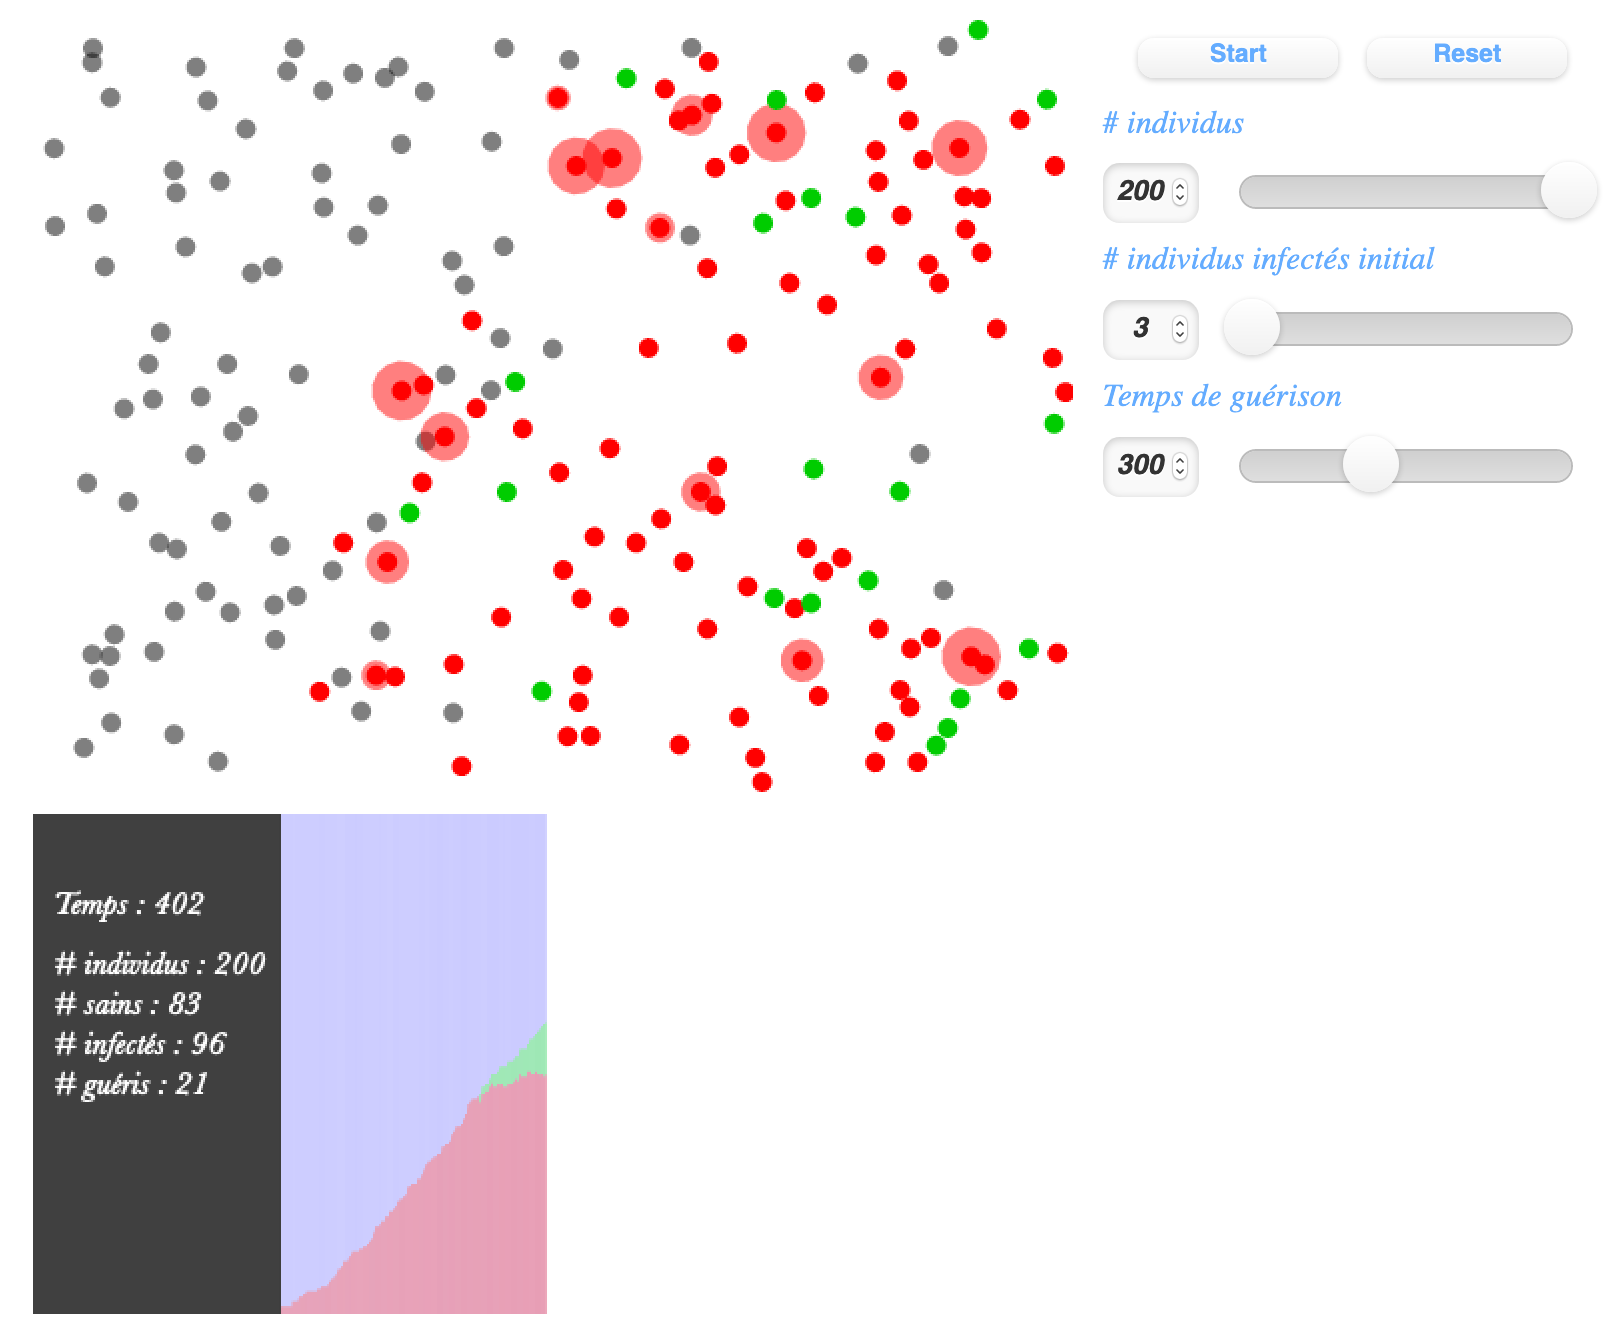
\includegraphics[width=0.6\linewidth]{approcheSMA.png} \\
        Approche individus
  \end{minipage}
  \
  
\end{frame}

% --------------------------------------


\begin{frame}
  \hfill \
  \begin{center}
    \Huge
    Notre situation actuelle
  \end{center}
  \hfill \

\end{frame}



% --------------------------------------

\begin{frame}[fragile]
  \frametitle{principes}
  \begin{itemize}
  \item Une approche par flux (compartiments) ``classique'' (Inserm ou Pasteur)
  \item SIGRM avec taux de transmission variable tout au long du temps
  \item SIAGRM (avec asymptomatiques et non asymptomatiques)
  \end{itemize}
  
\end{frame}



% --------------------------------------

\begin{frame}[fragile]
  \frametitle{La validation}
  \begin{itemize}
  \item Un modèle s'appuie sur des paramètres
  \item Plus il y a de paramètres plus c'est facile de coller aux données (overfitting)
  \end{itemize}

  \bigskip
  
  \textbf{Question : Comment valider le modèle}

  \begin{itemize}
  \item Par autorité
    
  \item par calibration
    \begin{itemize}
    \item Par les faits stylisés propres à une épidémie 
      (croissance exponentielle, puis décroissance)
    \item Par sa capacité à reproduire le passé (est-ce qu'on peut régler les paramètres pour que le modèle montre la situation actuelle)
  \end{itemize}

  \end{itemize}
\end{frame}


% --------------------------------------

\begin{frame}[fragile]
  \frametitle{Faits stylisés}
  
  \begin{center}
            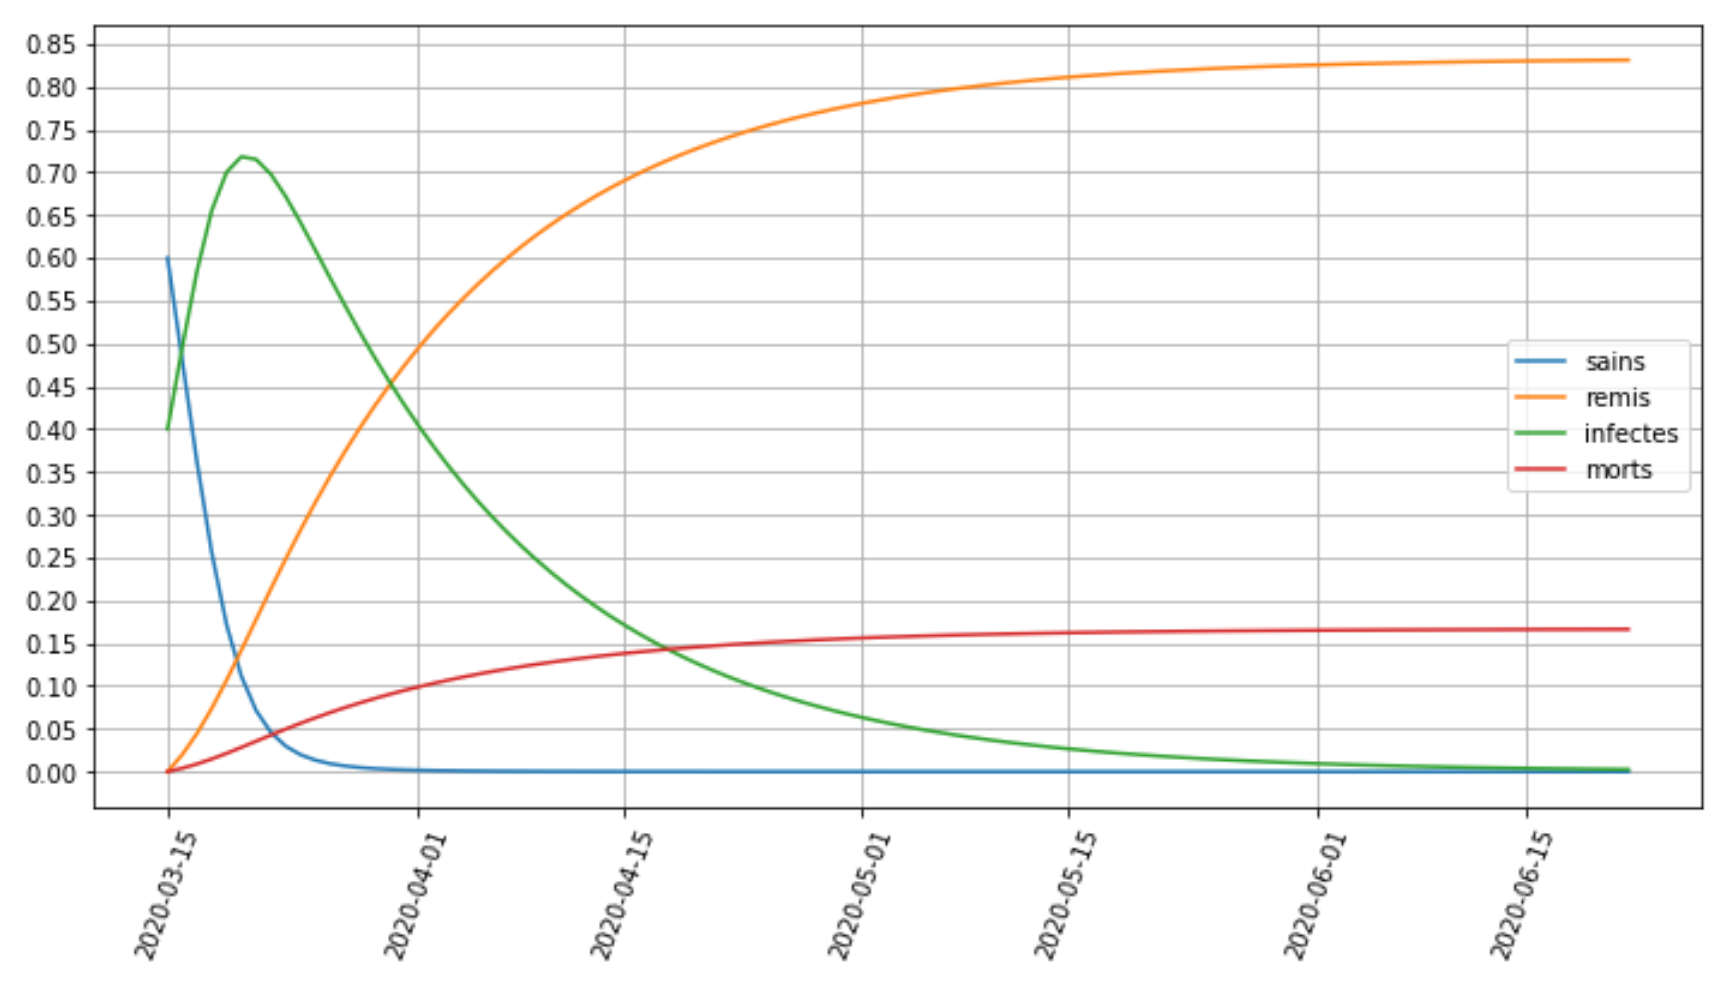
\includegraphics[width=0.6\linewidth]{fig3_sirgm.png} \\
  \end{center}

  
\end{frame}


% --------------------------------------

\begin{frame}[fragile]
  \frametitle{Coller à la situation actuelle}

  \begin{center}
    \includegraphics[width=0.6\linewidth]{} \\
    Courbe obtenue avec les données ministère santé \texttt{data.gouv.fr}
  \end{center}
  
\end{frame}



% --------------------------------------

\begin{frame}[fragile]
  \frametitle{Effet de différents confinements}


  \begin{center}
    \includegraphics[width=0.6\linewidth]{} \\
    Courbe obtenue avec les données ministère santé \texttt{data.gouv.fr}\\
    Courbe avec 2 bosses
  \end{center}
  
\end{frame}

% --------------------------------------

\begin{frame}[fragile]
  \frametitle{Des hypothèses optimistes et pessimistes}
  \begin{center}
        \includegraphics[width=0.6\linewidth]{} \\
  \end{center}
Fait avec les données régionales
  
\end{frame}


% --------------------------------------

\begin{frame}[fragile]
  \frametitle{Comparaison avec Pasteur}

  %\fbox{}
  \begin{minipage}[b]{0.45\columnwidth}
    \vspace{0.0cm}
    \includegraphics[width=\linewidth]{pasteur.png} \\
    Pasteur 
      \end{minipage}    
  \hfill \ 
  \begin{minipage}[b]{0.45\columnwidth}
        \vspace{0.0cm}
        \includegraphics[width=0.8\linewidth]{notrePasteur.png} \\
        Notre résultat
      \end{minipage}
      \

  Regardez ce qu'ils montrent .... regardez ce qu'on montre 
\end{frame}

% --------------------------------------

\begin{frame}[fragile]
  \frametitle{Comparaison avec Inserm}

  %\fbox{}
  \begin{minipage}[b]{0.45\columnwidth}
    \vspace{0.0cm}
    \includegraphics[width=\linewidth]{inserm.png} \\
    Inserm 
      \end{minipage}    
  \hfill \ 
  \begin{minipage}[b]{0.45\columnwidth}
        \vspace{0.0cm}
        \includegraphics[width=0.8\linewidth]{notreInserm.png} \\
        Notre résultat
      \end{minipage}
      \ 


  Regardez ce qu'ils montrent .... regardez ce qu'on montre 

\end{frame}


% --------------------------------------


\begin{frame}
  \hfill \
  \begin{center}
    \Huge
    Ce que nous souhaitons faire
  \end{center}
  \hfill \

\end{frame}

% --------------------------------------

\begin{frame}[fragile]
  \frametitle{Nous sommes complémentaires !}

  Il y a surement plein de biais ....On a besoin de collaborer

  \begin{itemize}
    \item On est juste des modélisateurs
    \item On a besoin de votre experience en termes de medecin
    \item Qu'est-ce que vous attendez de nous ?
    \end{itemize}

  
\end{frame}


\end{document}

